% reset section counter
%\setcounter{section}{0}

%\metadata{lecture ID}{Your names}{date}
\metadata{11}{Andrew Wang}{Feb 22nd, 2021}

\subsec{Matrix Completion \cite{ge2016}}
We consider rank-1 matrix completion for simplicity. Let $M = zz^\top$ be a rank-1 symmetric and positive semi-definite matrix for some $z\in \bbR^d$. Given random entries of $M$, our goal is to recover the rest of entries. Formally, we have the following definitions:

\begin{definition}
Suppose $M\in \bbR^{d\times d}$ and $\Omega \subseteq [d] \times [d]$, we define $P_{\Omega}(M)$ to be the matrix obtained by zeroing out every entry outside $\Omega$. 
\end{definition}

\begin{definition}[Matrix Completion]
Suppose $M\in \bbR^{d\times d}$ and every entry of $M$ is included in $\Omega$ with probability $p$. The \textit{matrix completion task} is to recover $M$ (with respect to some loss functions) given the observation $P_{\Omega}(M)$.
\end{definition}

A nice real world example of matrix completion is when we have a matrix describing the user ratings for each item. We only observe a small portion of the entries as each customer only buys a small subset of the items. A good matrix completion algorithm is indispensable for a recommendation engine. 

\begin{remark}
We need $d$ parameters to describe a rank-1 matrix $M$ and the number of observations is roughly $pd^2$. Thus, for identifiability we need to work in the regime where $pd^2 > d$, i.e. $p \gg \frac{1}{d}$. 
\end{remark}

We define our non-convex loss functions to be 
\begin{align}
    \min_{x \in \bbR^d} f(x) & \triangleq \frac{1}{2}\sum_{(i,j)\in \Omega}(M_{ij}-x_ix_j)^2 \\
     & = \frac{1}{2}\|P_{\Omega}(M-xx^\top)\|_F^2.
\end{align}

\tnote{does this \url{https://edstem.org/us/courses/14347/discussion/827805} means that we should update this section slightly to avoid the confusions? It perhaps doesn't take much to copy paste some of the texts in the answer to the notes?(I didn't read the question carefully enough though)}

To really solve our problem we need some regularity condition on the ground truth vector $z$ (recall $M = zz^\top$). \textit{Incoherence} is one such condition:
\begin{definition}[Incoherence]
Without loss of generality, assume the ground truth vector $z\in\bbR^d$ satisfies $\|z\|_2 = 1$. $z$ satisfies the \textit{incoherence condition} if $\|z\|_{\infty} \leq \frac{\mu}{\sqrt{d}}$, where $\mu$ is considered to be a constant or log in dimension $d$. 
\end{definition}

\begin{remark}
A nice counterexample to think about why such condition is necessary is when $z = e_1$ and $M = e_1 e_1^\top$. All entries of $M$ are 0 except for a 1 in the top-left corner. There is no way to recover $M$ without observing the top-left corner.
\end{remark}

The goal is to prove that local minima of this objective function are close to a global minimum:

\begin{theorem}\label{lec11:thm:matrix-completion}
Assume $p = \dfrac{\textrm{poly}(\mu, \log d)}{d\epsilon^2}$ for some sufficient small constant $\epsilon$ and assume $z$ is incoherent. Then with high probability, all local minima of $f$ are $O(\sqrt{\epsilon})$-close to $+z$ or $-z$ (the global minima of $f$).
\end{theorem}

Before presenting the proof, we make some observations that will guide the proof strategy.

\begin{remark}
$f(x)$ can be viewed as a sampled version of the PCA loss function $g(x) = \frac{1}{2}\norm{M - xx^\top}_F^2 = \frac{1}{2}\sum_{(i,j) \in [d]\times[d]} (M_{ij} - x_ix_j)^2$, in which we only observe a subset of the matrix entries. Thus, we would like to claim that $f(x) \approx g(x)$. However, matching the values of $f$ and $g$ is not sufficient to prove the theorem: even a small margin of error between $f$ and $g$ could lead to creation of many spurious local minima (see Figure~\ref{lec11:fig:matrix_completion_f_g} for an illustration). In order to ensure that the local minima of $f$ look like the local minima of $g$, we will need further conditions like $\nabla f(x) \approx \nabla g(x)$ and $\nabla^2 f(x) \approx \nabla^2 g(x)$.
\end{remark}

\begin{figure}
    \centering
    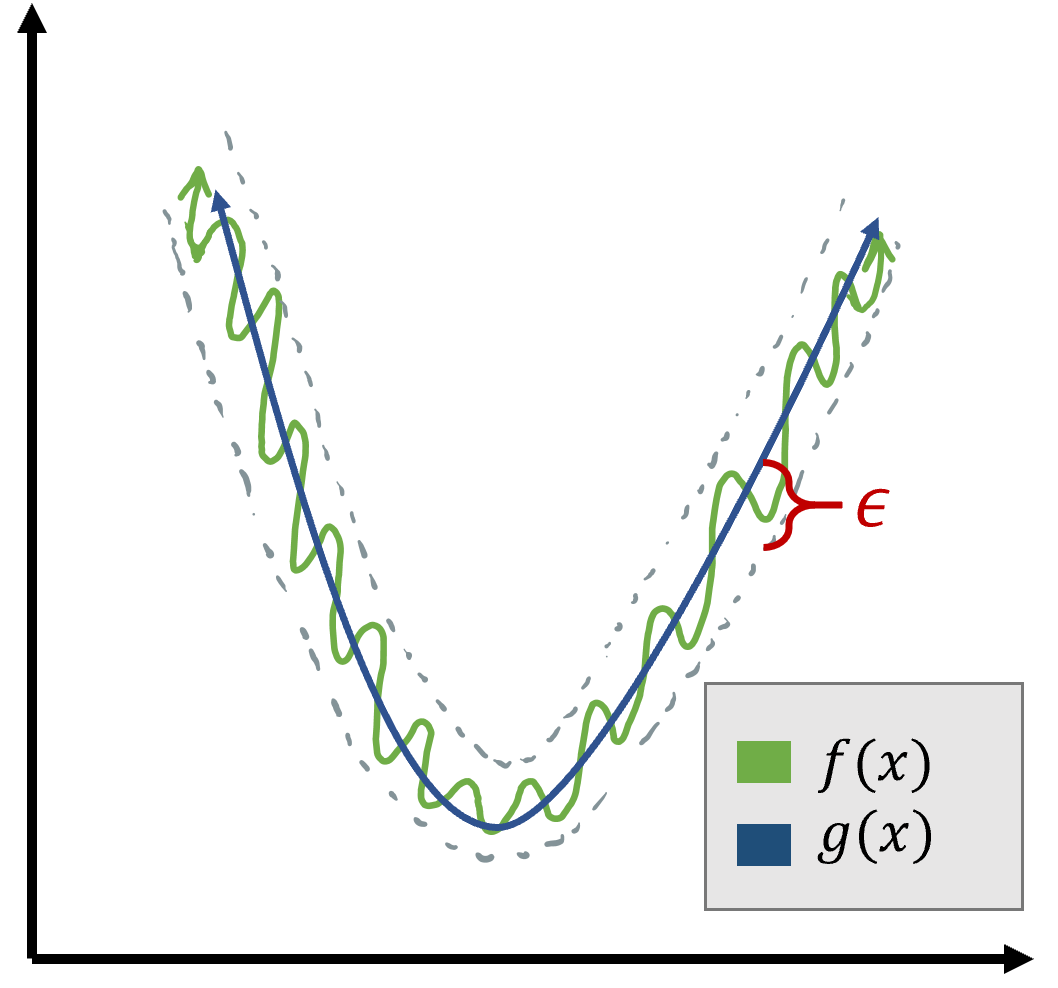
\includegraphics[width=2.5in]{figures/matrix-completion-f-g.png}
    \caption{Even if $f(x)$ and $g(x)$ are no more than $\epsilon$ apart at any given $x$, without any additional knowledge, the local minima of $f$ may possibly look dramatically different from the local minima of $g$. However, the proofs in this section show that the landscape of $f$ (the matrix completion objective) and $g$ (the PCA objective) are have similar properties by proving more advanced concentration inequalities. }
    \label{lec11:fig:matrix_completion_f_g}
\end{figure}

\begin{remark}
Key idea: concentration for scalars is easy. We can approximate a sum of scalars via a sample:
\begin{equation}
\sum_{(i,j) \in \Omega} T_{ij} \approx p\sum_{(i,j) \in [d]\times[d]} T_{ij},
\end{equation}
where we use $\approx$ to mean that
\begin{equation}
\Bigl| \sum_{(i,j) \in \Omega} T_{ij} - p\sum_{(i,j) \in [d]\times[d]} T_{ij} \Bigr| < \epsilon
\end{equation}
with high probability. This suggests the strategy of casting the estimation of our desired quantities in the form of estimating a scalar sum via a sample. In particular, we note that for any matrices $A$ and $B$,
\begin{equation}
\langle A, P_\Omega(B) \rangle = \sum_{(i,j) \in \Omega} A_{ij}B_{ij} \approx p\langle A, B \rangle.
\end{equation}
\end{remark}

To make use of this observation to understand the quantities of interest ($\nabla f(x)$ and $\nabla^2 f(x)$), we compute the bilinear and quadratic forms for $\nabla f(x)$ and $\nabla^2 f(x)$ respectively:
\begin{equation}
\langle v, \nabla f(x) \rangle = \langle v, P_\Omega(M-xx^\top)x \rangle = \langle vx^\top, P_\Omega(M-xx^\top) \rangle,
\end{equation}
where we have used the fact that $\langle A,BC \rangle = \langle AC^\top,B\rangle$. Also note that $vx^\top$ is a rank-1 matrix and $M-xx^\top$ is a rank-2 matrix.
\begin{align}
\langle v, \nabla^2 f(x) v \rangle &= \norm{P_\Omega(vx^\top + xv^\top)}_F^2 - 2\langle P_\Omega(M-xx^\top), vv^\top \rangle \\
&=  \langle P_\Omega(vx^\top + xv^\top), vx^\top + xv^\top \rangle - 2\langle P_\Omega(M-xx^\top), vv^\top \rangle,
\end{align}

where we have used the fact that $\norm{P_\Omega(A)}_F^2 = \langle P_\Omega(A), P_\Omega(A)\rangle = \langle P(\Omega(A), A\rangle$.

The key lemma that applies the scalar concentration to these matrix quantities is as follows:

\begin{lemma}
Let $\epsilon>0$, $p = \dfrac{\textrm{poly}(\mu, \log d)}{d\epsilon^2}$. Given that $A = uu^\top, B=vv^\top$ for some $u, v$ satisfying $\norm{u}_2 \leq 1$, $\norm{v}_2 \leq 1$, $\norm{u}_\infty \leq \mu / \sqrt{d}$, $\norm{v}_\infty \leq \mu / \sqrt{d}$, we have $|\langle P_\Omega(A), B \rangle/p - \langle A, B\rangle| \leq \epsilon$ w.h.p.
\label{lec11:lem:concentration_lemma}
\end{lemma}

If we can show that $g$ has no bad local minima via a proof that only uses $g$ via terms of the form $\langle v, \nabla g(x) \rangle$ and $\langle v, \nabla^2 g(x) v \rangle$, then by Lemma~\ref{lec11:lem:concentration_lemma} this proof will automatically generalize to $f$ by concentration.

Next, we prove some facts about $g$ and show the analogous proofs for $f$ that we will use in the proof of Theorem~\ref{lec11:thm:matrix-completion}.

\begin{lemma}[Connecting inner product and norm for $g$]\label{lec11:lem:inner-g}
If $x$ satisfies $\nabla g(x) = 0$, then $\langle x,z \rangle^2 = \norm{x}_2^4$.
\end{lemma}

\begin{proof}
\begin{align}
    \nabla g(x) = 0 &\implies \langle x, \nabla g(x) \rangle = 0 \\
   & \implies \langle x, (zz^\top-xx^\top)x \rangle = 0 & (\because \nabla g(x) = (M - xx^\top)x) \\
   & \implies \langle x,z \rangle^2 = \norm{x}_2^4.
\end{align}
\end{proof}

\begin{lemma}[Connecting inner product and norm for $f$]\label{lec11:lem:inner-f}
Suppose $\norm{x}_\infty \leq 2\mu / \sqrt{d}$. If $x$ satisfies $\nabla f(x) = 0$, then $\langle x,z \rangle^2 \geq \norm{x}_2^4 - \epsilon$ with high probability.
\label{inner_prod_norm_f}
\end{lemma}

\begin{proof}
\begin{align}
    \nabla f(x) = 0 &\implies \langle x, \nabla f(x) \rangle = 0 \\
    & \implies \langle x, \nabla g(x) \rangle \approx \langle x, \nabla f(x) \rangle/p \pm \epsilon & \text{(by Lemma \ref{lec11:lem:concentration_lemma})} \\
   & \implies |\langle x, (zz^\top-xx^\top)x \rangle| \leq \epsilon & \text{w.h.p.} \\
   & \implies \langle x,z \rangle^2 \geq \norm{x}_2^4 - \epsilon & \text{w.h.p.}
\end{align}
\end{proof}

\begin{lemma}[Bound norm for $g$]\label{lec11:lem:bound-g}
    If $\nabla^2 g(x) \succeq 0$, then $\norm{x}_2^2 \geq 1/3$.
\end{lemma}

\begin{proof}
\begin{align}
    \nabla^2 g(x) \succeq 0
    &\implies \langle z, \nabla^2 g(x)z\rangle \geq 0 \\
    &\implies \norm{zx^\top + xz^\top}_F^2 - 2z^\top(zz^\top-xx^\top)z \geq 0 \\
    &\implies 1 \leq \norm{x}_2^2 + 2\langle x,z \rangle^2 \leq \norm{x}_2^2 + 2\norm{x}_2^2 = 3\norm{x}_2^2 &\text{(by Cauchy-Schwarz)} \\
    &\implies \norm{x}_2^2 \geq 1/3.
\end{align}
\end{proof}

\begin{lemma}[Bound norm for $f$]\label{lec11:lem:bound-f}
    Suppose $\norm{x}_\infty \leq \mu / \sqrt{d}$. If $\nabla^2 f(x) \succeq 0$, then $\norm{x}_2^2 \geq 1/3 - \epsilon/3$ with high probability.
\end{lemma}
\begin{proof}
\begin{align}
    \nabla^2 f(x) \succeq 0
    &\implies \langle z, \nabla^2 f(x)z \rangle \geq 0 \\
    &\implies \langle z, \nabla^2g(x)z \rangle \geq -\epsilon & \text{w.h.p. (by Lemma \ref{lec11:lem:concentration_lemma})} \\
    &\implies 3\norm{x}_2^2 \geq 1-\epsilon & \text{w.h.p.} \\
    &\implies \norm{x}_2^2 \geq 1/3 - \epsilon/3 & \text{w.h.p.}
\end{align}
\end{proof}

\begin{lemma}[$g$ has no bad local minimum]
    All local minima of $g$ are global minima.
\end{lemma}

\begin{proof}
\begin{align}
    \nabla g(x) = 0
    & \implies \langle z, \nabla g(x) \rangle = 0 \\
    & \implies \langle z, (zz^\top-xx^\top)x \rangle = 0 \\
    & \implies \langle x,z\rangle (1-\norm{x}_2^2) = 0.
\end{align}
Since $|\langle x,z \rangle| \geq 1/3 \neq 0$ (by Lemma~\ref{lec11:lem:bound-g}), we must have $\norm{x}_2^2 = 1$. But then Lemma~\ref{lec11:lem:inner-g} implies $\langle x, z\rangle^2 = \norm{x}_2^4 = 1$, so $x = \pm z$ by Cauchy-Schwarz.
\end{proof}

We now prove Theorem~\ref{lec11:thm:matrix-completion}, restated for convenience:
\begin{theorem}[$f$ has no bad local minimum]
Assume $p = \dfrac{\textrm{poly}(\mu, \log d)}{d\epsilon^2}$. Then with high probability, all local minima of $f$ are $O(\sqrt{\epsilon})$-close to $+z$ or $-z$.
\end{theorem}

\begin{proof}
Observe that $\norm{x-z}_2^2 = \norm{x}_2^2 + \norm{z}_2^2 - 2\langle x,z \rangle \leq \norm{x}_2^2 + 1 - 2\langle x,z \rangle$. Our goal is to show that this quantity is small with high probability, hence we need to bound $\norm{x}_2^2$ and $\langle x,z \rangle$ w.h.p. Note that the following bounds in this proof are understood to hold w.h.p.
    
Let $x$ be such that $\nabla f(x) = 0$. For $\epsilon \leq 1/16$,
\begin{align}
\langle x,z \rangle^2 &\geq \norm{x}_2^4 - \epsilon &\text{(by Lemma~\ref{lec11:lem:inner-f})} \\
&\geq (1/3-\epsilon/3)^2 - \epsilon &\text{(by Lemma~\ref{lec11:lem:bound-f})} \\
&\geq 1/32. \label{lec11:eqn:xz-bound}
\end{align}

With this, we can get a bound on $\norm{x}_2^2$:
\begin{align}
\nabla f(x) = 0 &\implies \langle x, \nabla f(x) \rangle = 0 \\
&\implies |\langle z, \nabla g(x) \rangle| \leq \epsilon & \text{(by Lemma \ref{lec11:lem:concentration_lemma})} \\
&\implies |\langle x,z\rangle| \cdot |1-\norm{x}_2^2| \leq \epsilon &\text{(by dfn of $g$)} \\
&\implies |1-\norm{x}_2^2| \leq 32\epsilon = O(\epsilon) &\text{(by \eqref{lec11:eqn:xz-bound})} \\
&\implies \norm{x}_2^2 = 1 \pm O(\epsilon). \label{lec11:eqn:xnorm-bound}
\end{align}
    
Next, we bound $\langle x,z \rangle$:
\begin{align}
\langle x, z \rangle^2 &\geq \norm{x}_2^4 - \epsilon &\text{(by Lemma \ref{inner_prod_norm_f})} \\
&\geq (1-O(\epsilon))^2 - \epsilon &\text{(by \eqref{lec11:eqn:xnorm-bound})} \\
&= 1 - O(\epsilon).
\end{align}

Finally, we put these quantities together to bound $\norm{x-z}_2^2$. We have two cases:
    
\textbf{Case 1}: $\langle x,z\rangle \geq 1 - O(\epsilon)$. Then
\begin{align}
\norm{x-z}_2^2 &= \norm{x}_2^2 + \norm{z}_2^2 - 2\langle x,z \rangle \\
&\leq \norm{x}_2^2 + 1 - 2\langle x,z \rangle \\
&\leq 1 + O(\epsilon) + 1 - 2(1-O(\epsilon)) \\
&\leq O(\epsilon).
\end{align} 
    
Hence we conclude $x$ is $O(\sqrt{\epsilon})$-close to $z$.
    
\textbf{Case 2}: $\langle x,z\rangle \leq -(1 - O(\epsilon))$. Then by an analogous argument, $x$ is $O(\sqrt{\epsilon})$-close to $-z$.
\end{proof}

We have shown above that matrix completion of a rank-1 matrix has no spurious local minima. This proof strategy can be extended to handle higher-rank matrices and noisy matrices \cite{ge2016}. The proof also demonstrates a generally useful proof strategy: often, reducing a hard problem to an easy problem results in solutions that do not give much insight into the original problem, because the proof techniques do not generalize. It can often be fruitful to seek a proof in the simplified problem that makes use of a restricted set of tools that could generalize to the harder problem. Here we limited ourselves to only using $\langle v, \nabla g(x)\rangle$ and $\langle v, \nabla^2 g(x) v\rangle$ in the easy case; these quantities could then be easily converted to analogous quantities in $f$ via the concentration lemma (Lemma~\ref{lec11:lem:concentration_lemma}).

\subsec{Other problems where all local minima are global minima}
We have now demonstrated that two classes of machine learning problems, rank-1 PCA and rank-1 matrix completion, have no spurious local minima and are thus amenable to being solvable by gradient descent methods. We now outline some major classes of problems for which it is known that there are no spurious local minima.

\begin{itemize}
    \item Principal component analysis (covered in previous lecture).
    \item Matrix completion (and other matrix factorization problems). On a related note, it has also been shown that linearized neural networks of the form $y = W_1W_2x$, where $W_1$ and $W_2$ are optimized separately, have no spurious local minima \cite{baldi1989neural}. It should be noted that linearized neural networks are not very useful in practice since the advantage of optimizing $W_1$ and $W_2$ separately versus optimizing a single $W=W_1W_2$ is not clear.
    \item Tensor decomposition. The problem is as follows:
    \begin{align}
        \text{maximize }\quad \sum_{i=1}^d \sum_{j=1}^d \sum_{k=1}^d \sum_{l=1}^d T_{ijkl} x_ix_jx_kx_l \quad \text{such that } \quad \norm{x}_2 = 1.
    \end{align}
    Additionally, constraints are imposed on the tensor $T$ to make the problem tractable. For example, one condition is that $T$ must be a low-rank tensor with orthonormal components \cite{ge2015}.
\end{itemize}